\documentclass[11pt]{article}

\usepackage[T1]{fontenc}
\usepackage[utf8]{inputenc}
\usepackage{lmodern}
\usepackage[a4paper,margin=1in]{geometry}
\usepackage{amsmath,amssymb}
\usepackage{enumitem}
\usepackage{booktabs}
\usepackage{xcolor}
\usepackage{tikz}
\usepackage{hyperref}
\usetikzlibrary{arrows.meta,positioning,calc,fit,backgrounds}

\hypersetup{colorlinks=true,linkcolor=blue!70!black,urlcolor=blue!70!black}

% ── one running palette of colours, used everywhere ─────────────────────────────
\definecolor{col1}{RGB}{229,115,115}   % colour 1  (red)
\definecolor{col2}{RGB}{100,181,246}   % colour 2  (blue)
\definecolor{col3}{RGB}{255,213,79}    % colour 3  (yellow)

\tikzset{
  v/.style   ={circle,draw,thick,minimum size=8mm,inner sep=0pt,font=\scriptsize},
  slot/.style={circle,draw,thick,minimum size=8mm,inner sep=0pt,font=\scriptsize},
  pick/.style={circle,draw,thick,fill=green!30,minimum size=8mm,inner sep=0pt,font=\scriptsize},
  sep/.style ={circle,draw,thick,fill=orange!35,minimum size=8mm,inner sep=0pt,font=\scriptsize},
  log/.style ={circle,draw,thick,fill=white,minimum size=8mm,inner sep=0pt,font=\scriptsize},
  gat/.style ={circle,draw,fill=gray!25,minimum size=5mm,inner sep=0pt,font=\tiny},
  cc1/.style ={fill=col1!70}, cc2/.style={fill=col2!70}, cc3/.style={fill=col3!80},
  choice/.style ={gray,thick},
  conflict/.style={red!60!black,thick,dashed},
  ar/.style={-{Stealth[length=2.4mm]},thick},
}

% a friendly highlighted "key idea" box that needs no extra packages
\newcommand{\idea}[1]{%
  \par\smallskip\noindent
  \fcolorbox{black}{yellow!14}{%
    \parbox{\dimexpr\linewidth-2\fboxsep-2\fboxrule\relax}{\textbf{In plain words.}\ #1}}%
  \par\smallskip}

\title{\textbf{The Whole Pipeline, Explained Gently}\\[0.4em]
  \large From colouring a graph to lighting up atoms --- and back again}
\author{A plain-language companion to the paper}
\date{\today}

\begin{document}
\maketitle

\begin{abstract}
\noindent This note explains, in the simplest terms I can manage, every step that
turns a graph-colouring question into something a neutral-atom machine can solve,
and how we read the answer back out. We follow \emph{one tiny example} the whole
way through. No proofs, no heavy notation --- just what each step does and why.
The order is the order the machine sees it: colouring $\to$ independent set $\to$
gadget $\to$ the seven layout heuristics $\to$ decomposition (for big graphs)
$\to$ recovering the colours.
\end{abstract}

\tableofcontents

% =============================================================================
\section{The journey in one breath}
% =============================================================================

We want to \textbf{colour the vertices of a graph} with $k$ colours so that no
edge joins two same-coloured vertices. The hardware cannot do this directly. It
can only do \emph{one} thing: take a bunch of atoms placed in the plane and find
the heaviest set of atoms with no two of them sitting close together. So we
translate, in three exact steps, and one geometric step:

\begin{center}
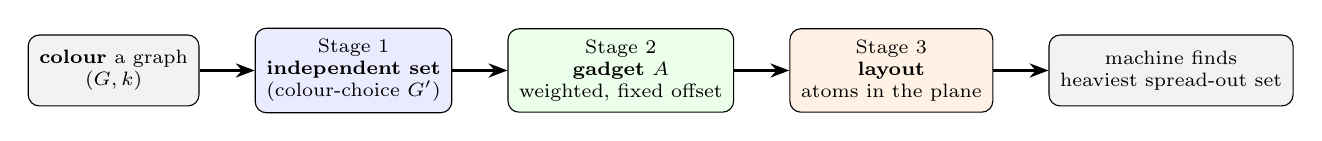
\begin{tikzpicture}[font=\scriptsize,node distance=5mm,
  b/.style={rectangle,draw,rounded corners,minimum height=9mm,align=center,inner sep=4pt}]
  \node[b,fill=gray!10]  (G)   {\textbf{colour} a graph\\ $(G,k)$};
  \node[b,fill=blue!8,right=7mm of G]  (is) {Stage 1\\ \textbf{independent set}\\ (colour-choice $G'$)};
  \node[b,fill=green!8,right=7mm of is] (gad){Stage 2\\ \textbf{gadget} $A$\\ weighted, fixed offset};
  \node[b,fill=orange!10,right=7mm of gad](lay){Stage 3\\ \textbf{layout}\\ atoms in the plane};
  \node[b,fill=gray!10,right=7mm of lay] (hw) {machine finds\\ heaviest spread-out set};
  \draw[ar](G)--(is); \draw[ar](is)--(gad); \draw[ar](gad)--(lay); \draw[ar](lay)--(hw);
\end{tikzpicture}
\end{center}

\idea{Stages 1 and 2 are \emph{exact} translations --- they never change the
answer, only its form. Stage 3 is \emph{geometry} --- it decides whether the
machine can physically fit the problem, but it can never give a wrong colour.
At the end we run the arrows backwards to read the colours off.}

\paragraph{Our running example.} The smallest graph that shows everything: a path
of three vertices, $a-b-c$, and we ask for a \textbf{2-colouring}
($k=2$, colours $1$ and $2$).

\begin{center}
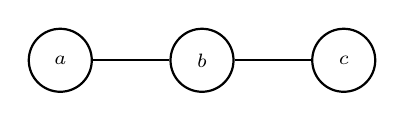
\begin{tikzpicture}[scale=1]
  \node[v] (a) at (0,0){$a$};
  \node[v] (b) at (1.8,0){$b$};
  \node[v] (c) at (3.6,0){$c$};
  \draw[thick] (a)--(b)--(c);
\end{tikzpicture}
\end{center}

\noindent An obvious answer is $a=1,\ b=2,\ c=1$. Let us watch the machinery
rediscover it.

% =============================================================================
\section{Stage 1: colouring $\to$ independent set (the colour-choice graph)}
% =============================================================================

\textbf{The trick.} Make one little ``light switch'' for every (vertex, colour)
pair. The switch $(v,i)$ means \emph{``vertex $v$ takes colour $i$.''} For our
example with $2$ colours that is $3\times 2 = 6$ switches. Now we wire them with
two kinds of \emph{forbidding} edges:

\begin{itemize}[leftmargin=1.6em,itemsep=2pt]
  \item \textbf{Choice edges} (one column per vertex): the two switches of the
        same vertex are joined, because a vertex may take \emph{at most one}
        colour. You cannot turn on both $(a,1)$ and $(a,2)$.
  \item \textbf{Conflict edges} (between neighbours): if $a-b$ is an edge of the
        graph, join $(a,1)$ to $(b,1)$ and $(a,2)$ to $(b,2)$, because
        neighbours may \emph{not} share a colour. You cannot turn on $(a,1)$ and
        $(b,1)$ together.
\end{itemize}

This wired-up graph is the \textbf{colour-choice graph} $G'$. A set of switches
with \emph{no forbidding edge between any two of them} is exactly an
\emph{independent set}.

\begin{center}
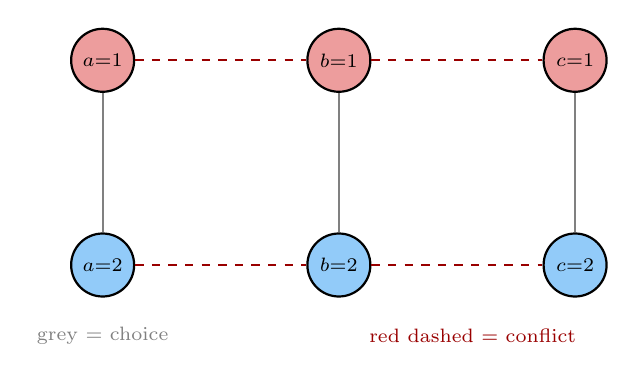
\begin{tikzpicture}[scale=1]
  % columns a,b,c ; rows colour1 (top), colour2 (bottom)
  \node[slot,cc1] (a1) at (0,1.3){$a{=}1$};
  \node[slot,cc2] (a2) at (0,-1.3){$a{=}2$};
  \node[slot,cc1] (b1) at (3,1.3){$b{=}1$};
  \node[slot,cc2] (b2) at (3,-1.3){$b{=}2$};
  \node[slot,cc1] (c1) at (6,1.3){$c{=}1$};
  \node[slot,cc2] (c2) at (6,-1.3){$c{=}2$};
  % choice edges (vertical, grey)
  \draw[choice] (a1)--(a2); \draw[choice] (b1)--(b2); \draw[choice] (c1)--(c2);
  % conflict edges (same row between neighbours, red dashed)
  \draw[conflict] (a1)--(b1); \draw[conflict] (b1)--(c1);
  \draw[conflict] (a2)--(b2); \draw[conflict] (b2)--(c2);
  \node[font=\scriptsize,gray] at (0,-2.2){\textcolor{gray}{grey = choice}};
  \node[font=\scriptsize] at (4.7,-2.2){\textcolor{red!60!black}{red dashed = conflict}};
\end{tikzpicture}
\end{center}

\idea{A \emph{proper $k$-colouring} of the original graph is the \emph{same thing}
as an independent set that switches on \emph{exactly one switch per vertex}
(that is, a set of size $n$). ``Colour the graph'' has become ``find a big
independent set.''}

\paragraph{Reading our example.} Turn on $(a{=}1)$, $(b{=}2)$, $(c{=}1)$:

\begin{center}
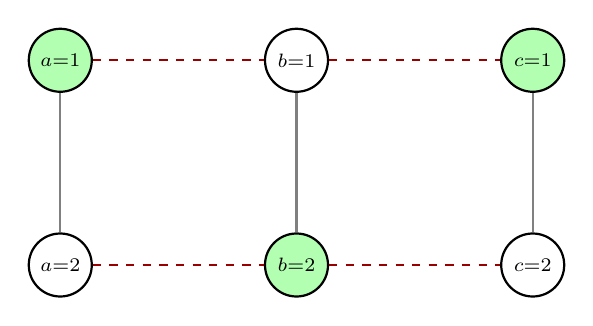
\begin{tikzpicture}[scale=1]
  \node[pick] (a1) at (0,1.3){$a{=}1$};
  \node[slot] (a2) at (0,-1.3){$a{=}2$};
  \node[slot] (b1) at (3,1.3){$b{=}1$};
  \node[pick] (b2) at (3,-1.3){$b{=}2$};
  \node[pick] (c1) at (6,1.3){$c{=}1$};
  \node[slot] (c2) at (6,-1.3){$c{=}2$};
  \draw[choice] (a1)--(a2); \draw[choice] (b1)--(b2); \draw[choice] (c1)--(c2);
  \draw[conflict] (a1)--(b1); \draw[conflict] (b1)--(c1);
  \draw[conflict] (a2)--(b2); \draw[conflict] (b2)--(c2);
\end{tikzpicture}
\end{center}

No two green switches are joined: $(a{=}1)$ and $(b{=}2)$ are in different rows
(no conflict), $a$ and $c$ are not neighbours, and we used one switch per column.
Three switches on $=$ three vertices coloured $=$ a valid $2$-colouring. If the
graph had \emph{needed} more colours, no size-$3$ independent set would exist, and
that is how the machine would say ``impossible.''

\medskip
\noindent\emph{(In the code this is \texttt{UDGColor.Stage1.colorChoiceGraph}; the
size of the biggest independent set is checked against a brute-force oracle on all
small graphs.)}

% =============================================================================
\section{Stage 2: independent set $\to$ gadget (the weighted graph $A$)}
% =============================================================================

The machine does not solve plain ``independent set''; it solves
\textbf{maximum-\emph{weight} independent set} (MWIS) on a graph where every edge
must come from atoms being physically close. Stage 2 rebuilds $G'$ into a weighted
graph $A$ that the machine likes, \emph{without changing which independent sets
win.}

\paragraph{The gadget, on one edge.} Replace each forbidding edge $\{u,v\}$ of
$G'$ by a little \textbf{chain of four}: keep the two original switches (now
called \emph{logical atoms}, weight~$1$) and insert two new helper atoms between
them (\emph{gadget atoms}, weight~$2$):

\begin{center}
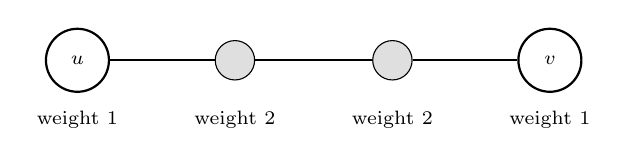
\begin{tikzpicture}[scale=1]
  \node[log] (u) at (0,0){$u$};
  \node[gat] (g1) at (2,0){};
  \node[gat] (g2) at (4,0){};
  \node[log] (v) at (6,0){$v$};
  \draw[thick] (u)--(g1)--(g2)--(v);
  \node[font=\scriptsize] at (0,-0.75){weight $1$};
  \node[font=\scriptsize] at (2,-0.75){weight $2$};
  \node[font=\scriptsize] at (4,-0.75){weight $2$};
  \node[font=\scriptsize] at (6,-0.75){weight $1$};
\end{tikzpicture}
\end{center}

Why four in a chain? Look at how much weight this little chain can contribute to a
spread-out (independent) set:

\begin{itemize}[leftmargin=1.6em,itemsep=2pt]
  \item Take \emph{one} helper atom: weight $2$. (The two helpers are joined, so
        you cannot take both.)
  \item You may also take \emph{one} of the end switches alongside a helper, as
        long as they are not adjacent --- so a single chain happily gives you
        weight $2$ plus maybe an endpoint.
  \item But if you greedily grab \emph{both} end switches $u$ \emph{and} $v$, the
        chain forces you to drop \emph{both} helpers, and you lose that weight-$4$
        of helpers to gain weight-$2$ of endpoints. Bad trade.
\end{itemize}

So the chain quietly \emph{punishes} taking both endpoints --- which is exactly
the old forbidding edge ``you may not take both $u$ and $v$,'' now enforced by
weights instead of a hard rule.

\idea{Every edge-chain pays the machine a fixed bonus no matter what, \emph{unless}
you try to switch on both of its endpoints. Add up the bonuses and you get a fixed
number $C=2\times(\text{number of edges of }G')$. The heaviest set of $A$ is then
the best independent set of $G'$ \emph{plus} that constant:
\[
   \text{MWIS}(A)\;=\;\alpha(G')\;+\;C.
\]
The constant carries no information; we just subtract it back off at the end.}

\paragraph{Our example by the numbers.} The colour-choice graph $G'$ of the path
has $7$ forbidding edges, so we build $7$ chains: $6$ logical atoms
$+\,2\times 7 = 14$ helper atoms $=\mathbf{20}$ atoms, and the offset is
$C = 2\times 7 = \mathbf{14}$. The best independent set of $G'$ has size $3$
(our colouring), so the machine's heaviest set weighs $3+14 = \mathbf{17}$.

\paragraph{Decoding is trivial.} From the heaviest set, \textbf{throw away the
helper atoms and keep the logical ones}. The logical atoms that survive are
exactly the switches we turned on --- our independent set, i.e.\ our colouring.

\medskip
\noindent\emph{(Code: \texttt{UDGColor.Gadget.gadgetize} and
\texttt{decodeLogical}; the identity $\text{MWIS}(A)=\alpha(G')+C$ is checked
against the oracle on all small graphs.)}

% =============================================================================
\section{Stage 3: the layout --- and the seven heuristics}
% =============================================================================

Up to now $A$ is just an abstract graph: ``these atoms are joined, those are
not.'' But the machine has no wires. Two atoms are joined \emph{only if they are
physically close} --- within a fixed \textbf{blockade radius} $r$. So we must
\textbf{place every atom of $A$ at a point in the plane} so that:

\begin{itemize}[leftmargin=1.6em,itemsep=1pt]
  \item every pair the gadget \emph{wants} joined ends up \emph{within} $r$
        (a \textbf{realized} edge), and
  \item every pair it wants \emph{apart} ends up \emph{farther} than $r$;
        if two atoms are accidentally too close, that is a \textbf{false edge},
        and if a wanted pair is too far, that is a \textbf{missing edge}.
\end{itemize}

\begin{center}
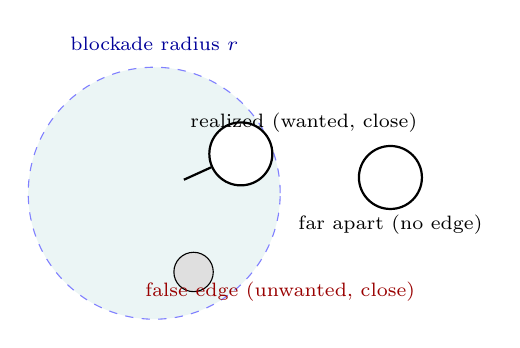
\begin{tikzpicture}[scale=1]
  \node[log] (p) at (0,0){};
  \draw[blue!50,dashed,fill=teal!8] (0,0) circle (1.6);
  \node[log] (q) at (1.1,0.5){};     % inside: a good (realized) neighbour
  \node[gat] (s) at (0.5,-1.0){};    % inside: too close -> false edge if not wanted
  \node[log] (far) at (3.0,0.2){};   % outside: far, no edge
  \draw[thick] (p)--(q);
  \node[font=\scriptsize,blue!60!black] at (0,1.9){blockade radius $r$};
  \node[font=\scriptsize] at (1.9,0.9){realized (wanted, close)};
  \node[font=\scriptsize,red!60!black] at (1.6,-1.25){false edge (unwanted, close)};
  \node[font=\scriptsize] at (3.0,-0.4){far apart (no edge)};
\end{tikzpicture}
\end{center}

\idea{This is the \emph{only} job of the heuristics: \textbf{geometry}. Because
Stage 2 already fixed the right answer exactly, a clumsy layout can only make the
problem \emph{not fit} or \emph{harder to solve} --- it can \textbf{never} produce
a wrong colour. That is the whole reason we were allowed to demote the heuristics
to ``helpers'' instead of trusting them with correctness.}

\paragraph{The seven heuristics, one by one.} They cooperate to find good atom
positions $p$ and a good radius $r$. Here is what each one actually does, in
plain terms (and roughly the order they run).

\begin{description}[leftmargin=0pt,itemsep=4pt]
\item[\textcolor{blue!60!black}{H4 --- smart starting positions} (runs first).]
  Don't start atoms randomly. Use the graph's own ``shape'' (its
  \emph{Laplacian eigenvectors}, a standard way to spread a graph out) to drop
  every atom roughly where it belongs: joined atoms start near each other,
  unrelated atoms start far apart. A good start saves the next step a lot of work.
  \emph{(Code: \texttt{fiedlerInit}.)}

\item[\textcolor{blue!60!black}{H1 --- nudge until it fits} (the main loop).]
  Treat wanted pairs like little springs pulling close and unwanted-but-too-close
  pairs like magnets pushing apart, plus a gentle floor that keeps no two atoms
  on top of each other. Then \emph{nudge} every atom a tiny step downhill,
  repeatedly, lowering a single ``badness'' score. We take a fixed number of
  steps (not ``until it magically converges''), and each step is checked so the
  score truly goes down. \emph{(Code: \texttt{descend}; in our example the score
  falls steadily over the allotted steps.)}

\item[\textcolor{blue!60!black}{H2 --- spend effort where it hurts.}]
  Some wanted connections have to snake through many other gadgets and are the
  expensive, error-prone ones. Weight those more heavily in the badness score, so
  the nudging focuses on tidying the long, tangled routes rather than the easy
  short ones.

\item[\textcolor{blue!60!black}{H3 --- don't let atoms pile up.}]
  A clump of atoms all within $r$ of each other creates a storm of false edges and
  wastes hardware. Detect over-crowded neighbourhoods and push the offenders
  apart. The physics even gives a hard ceiling on how many atoms can legally sit
  inside one blockade disk, which we respect.

\item[\textcolor{blue!60!black}{H5 --- local touch-ups that must improve.}]
  After the big nudging, a few stubborn bad pairs may remain. Fix them one at a
  time by sliding the two atoms along the line between them --- but only \emph{keep}
  a move if it strictly lowers the \emph{count of broken pairs}. Since that count
  is a whole number that can only go down, this is guaranteed to stop; it cannot
  loop forever. \emph{(Code: \texttt{repair}.)}

\item[\textcolor{blue!60!black}{H6 --- pick the radius.}]
  With the atoms placed, choose the smallest radius $r^\star$ that still captures
  \emph{every} wanted edge: $r^\star = $ the longest wanted-pair distance. Any
  smaller and we would lose a needed edge; we report this $r^\star$ and how many
  false edges it brings in. \emph{(Code: \texttt{minFeasibleRadius}.)}

\item[\textcolor{blue!60!black}{H7 --- judge, don't optimise, the discrete stuff.}]
  Counts like ``number of false edges'' jump in steps and have no smooth slope, so
  you cannot nudge them directly. Instead we use them only to \emph{score and
  compare} finished layouts (e.g.\ at the H6 radius choice), never as the thing
  H1 nudges. \emph{(Code: \texttt{falseEdges}, \texttt{missingEdges}.)}
\end{description}

\begin{center}
\renewcommand{\arraystretch}{1.15}
\begin{tabular}{@{}llp{6.6cm}@{}}
\toprule
 & role & one-line summary \\
\midrule
H4 & start  & place atoms using the graph's natural shape \\
H1 & drive  & nudge atoms downhill on a smooth badness score \\
H2 & weight & put the effort into the long, tangled connections \\
H3 & spread & break up over-crowded clumps of atoms \\
H5 & repair & local moves that must lower the broken-pair count \\
H6 & radius & smallest $r$ that keeps every wanted edge \\
H7 & judge  & use discrete quality only to compare layouts \\
\bottomrule
\end{tabular}
\end{center}

\paragraph{Our example, laid out.} For the path's gadget the layout actually
succeeds \emph{perfectly}: all wanted edges realized, \textbf{zero false edges,
zero missing}, at radius $r^\star=1.3$. (Bigger, denser instances leave some false
edges behind --- that residue is the honest signal that a truly clean placement
needs the specialised ``crossing gadgets'' we have not built yet. The heuristics
report the residue; they never hide it.)

\idea{Remember: even if the layout were ugly and full of false edges, the
\emph{colour we eventually read out is still correct or the layout is rejected as
infeasible} --- never silently wrong. Geometry decides ``does it fit,'' not ``what
is the answer.''}

% =============================================================================
\section{Decomposition: how to colour a graph too big for the machine}
% =============================================================================

The catch: the gadget's atom count grows like $(nk)^2$, so a few-hundred-atom
machine runs out of room after only a handful of vertices. The fix uses a simple
fact: \textbf{colouring is local.} Every rule is a single edge, and edges live
inside small neighbourhoods. So cut the graph into small \emph{overlapping pieces},
colour them \emph{one at a time}, and glue the results. The machine only ever
holds one small piece.

\paragraph{Cut at a separator.} A \emph{separator} is a small set of vertices
whose removal splits the graph in two. The friendliest kind is a
\emph{clique separator} (the shared vertices are all mutually adjacent), because
then gluing is free --- explained below.

\paragraph{Example: the bowtie.} Two triangles sharing a single vertex $c$. That
shared vertex is a separator of size one (a cut vertex).

\begin{center}
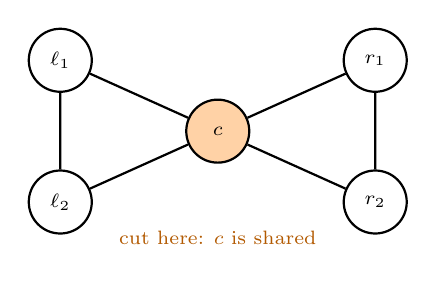
\begin{tikzpicture}[scale=1]
  \node[v] (l1) at (-2,0.9){$\ell_1$};
  \node[v] (l2) at (-2,-0.9){$\ell_2$};
  \node[sep] (c) at (0,0){$c$};
  \node[v] (r1) at (2,0.9){$r_1$};
  \node[v] (r2) at (2,-0.9){$r_2$};
  \draw[thick] (l1)--(l2)--(c)--(l1);
  \draw[thick] (r1)--(r2)--(c)--(r1);
  \node[font=\scriptsize,orange!70!black] at (0,-1.35){cut here: $c$ is shared};
\end{tikzpicture}
\end{center}

\paragraph{Step 1 --- solve the left triangle on its own.} Run the whole Stage
1--3 pipeline on just $\{\ell_1,\ell_2,c\}$ with $k=3$. The machine returns, say,
\[
   c=\textcolor{col1!85!black}{1},\quad \ell_1=\textcolor{col2!85!black}{2},\quad \ell_2=\textcolor{col3!72!black}{3}.
\]
The device only ever saw a $3$-vertex piece, not the whole graph.

\paragraph{Step 2 --- solve the right triangle, with $c$ pinned.} Now $c$ already
has colour $\textcolor{col1}{1}$. We \emph{precolour} it: in the colour-choice
graph of the right triangle, vertex $c$ keeps \emph{only} its switch $(c,1)$ and
loses the others. Solve; the machine fills in the rest, e.g.\
$r_1=\textcolor{col2!85!black}{2},\ r_2=\textcolor{col3!72!black}{3}$.

\paragraph{Step 3 --- glue.} Both pieces now agree that $c$ is colour
$\textcolor{col1}{1}$, so their colourings simply merge:

\begin{center}
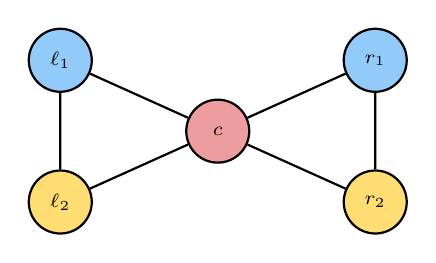
\begin{tikzpicture}[scale=1]
  \node[v,cc2] (l1) at (-2,0.9){$\ell_1$};
  \node[v,cc3] (l2) at (-2,-0.9){$\ell_2$};
  \node[v,cc1] (c) at (0,0){$c$};
  \node[v,cc2] (r1) at (2,0.9){$r_1$};
  \node[v,cc3] (r2) at (2,-0.9){$r_2$};
  \draw[thick] (l1)--(l2)--(c)--(l1);
  \draw[thick] (r1)--(r2)--(c)--(r1);
\end{tikzpicture}
\end{center}

\idea{\textbf{Why clique separators glue for free.} On the shared clique, every
two vertices are adjacent, so any valid colouring gives them \emph{all different}
colours. Two pieces might have used different \emph{names} for those colours, but
a colouring is only fixed up to renaming --- so we just relabel one piece's
colours to match the other on the shared vertices. No searching, no guessing.}

\paragraph{When the shared vertices are \emph{not} all adjacent.} Then renaming
isn't enough: we have to \emph{try} the possible colourings of the (small)
separator --- at most $k^{(\text{separator size})}$ of them --- and keep one that
works on both sides. Small separators keep this cheap; clique separators make it
vanish. Either way, \textbf{the machine never holds more than one piece}, so its
size depends on the biggest piece, not on how many vertices the whole graph has.
A chain of $1000$ triangles is coloured by $1000$ tiny three-vertex solves.

\medskip
\noindent\emph{(In the code, the precolouring already exists as
\texttt{colorChoiceGraphPrecolored}; the piece-cutting and stitching driver is the
next layer to build.)}

% =============================================================================
\section{Recovering the colours: running every arrow backwards}
% =============================================================================

Finally, the part that ties it all together --- turning the machine's raw output
back into colours on the \emph{original} graph. It is just every step undone, in
reverse:

\begin{center}
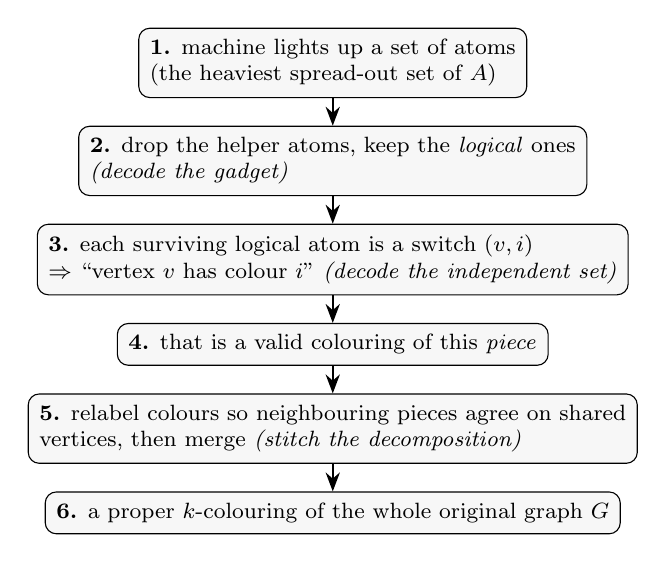
\begin{tikzpicture}[font=\footnotesize,node distance=3.5mm,
  s/.style={rectangle,draw,rounded corners,align=left,inner sep=4pt,fill=gray!6}]
  \node[s] (m)  {\textbf{1.} machine lights up a set of atoms\\ (the heaviest spread-out set of $A$)};
  \node[s,below=of m] (l) {\textbf{2.} drop the helper atoms, keep the \emph{logical} ones\\ \emph{(decode the gadget)}};
  \node[s,below=of l] (sw){\textbf{3.} each surviving logical atom is a switch $(v,i)$\\ $\Rightarrow$ ``vertex $v$ has colour $i$'' \emph{(decode the independent set)}};
  \node[s,below=of sw] (p){\textbf{4.} that is a valid colouring of this \emph{piece}};
  \node[s,below=of p] (g){\textbf{5.} relabel colours so neighbouring pieces agree on shared\\ vertices, then merge \emph{(stitch the decomposition)}};
  \node[s,below=of g] (f){\textbf{6.} a proper $k$-colouring of the whole original graph $G$};
  \draw[ar](m)--(l); \draw[ar](l)--(sw); \draw[ar](sw)--(p);
  \draw[ar](p)--(g); \draw[ar](g)--(f);
\end{tikzpicture}
\end{center}

\noindent And one bookkeeping detail: any vertices we peeled off at the start
because they had fewer than $k$ neighbours (they can always be coloured last) get
their colours filled in greedily at the very end --- there is always a free colour
left for them.

\idea{Each arrow we built going \emph{down} (Stages 1, 2, 3, and the cut) has a
matching arrow going \emph{up} that recovers the answer. The exact stages
(1 and 2) recover it perfectly; the layout (3) is just thrown away once the
machine has measured; and the decomposition glue (the cut) is undone by a cheap
colour-relabelling. That round trip --- a problem compiled down and an answer
certified back up --- is the whole point of the project.}

% =============================================================================
\section*{One-page recap}
\addcontentsline{toc}{section}{One-page recap}
% =============================================================================

\begin{enumerate}[leftmargin=1.6em,itemsep=2pt]
  \item \textbf{Colour $\to$ independent set.} Make a switch $(v,i)$ for each
        vertex/colour; forbid two colours on one vertex (choice) and the same
        colour on neighbours (conflict). A colouring $=$ an independent set of
        size $n$.
  \item \textbf{Independent set $\to$ gadget.} Replace each forbidding edge by a
        weight-$1$/weight-$2$ chain of four. The heaviest spread-out set is the
        best independent set plus a fixed constant $C$. Decode by keeping the
        logical atoms.
  \item \textbf{Gadget $\to$ layout.} Place the atoms in the plane so close pairs
        are exactly the wanted edges. Seven heuristics (start, drive, weight,
        spread, repair, radius, judge) handle the geometry --- and geometry alone.
  \item \textbf{Big graphs $\to$ pieces.} Cut at small separators, solve pieces one
        at a time with shared vertices pinned, glue by relabelling colours.
  \item \textbf{Read it back.} Lit atoms $\to$ logical atoms $\to$ switches $\to$
        piece colourings $\to$ stitched colouring of $G$.
\end{enumerate}

\end{document}
